\documentclass[12pt]{article}
\usepackage[english]{babel}
\usepackage[utf8]{inputenc}
\usepackage{amsmath,amssymb}
\usepackage{graphicx}
\usepackage{hyperref}
\usepackage{booktabs}
\usepackage{pgfplots}
\pgfplotsset{compat=1.18}
\usepackage{helvet}
\renewcommand{\familydefault}{\sfdefault}
\usepackage{setspace}
\onehalfspacing
\usepackage{geometry}
\geometry{
    left=2.5cm,
    right=2.5cm,
    top=2.5cm,
    bottom=2.5cm
}
\usepackage{ragged2e}
\justifying

\title{The Dutch Merchant Problem: A Complete Algorithmic Analysis}
\author{}
\date{}

\begin{document}

\maketitle

\begin{abstract}
This document presents a comprehensive analysis of the Dutch Merchant Problem, a combinatorial optimization problem that combines routing decisions with transaction optimization under multiple constraints. The work covers four main phases: (1) formal problem definition and mathematical modeling, (2) computational complexity analysis establishing NP-Completeness via reduction from Prize-Collecting TSP, (3) design and implementation of both exact brute force algorithms and efficient heuristic solutions, and (4) extensive experimental evaluation comparing solution quality and performance. The exact algorithms (pure brute force, pruned brute force, and hybrid brute force with dynamic programming) serve as optimal baselines for small instances ($n \leq 11$), while the two-phase hybrid algorithm (beam search route generation with multi-dimensional dynamic programming) efficiently handles medium-to-large instances ($15 \leq n \leq 30$) with multiple item types and $k$-unit operations. Experimental results demonstrate exponential growth in exact methods, validate the efficiency of the heuristic approach, and provide insights into algorithm behavior across different instance characteristics.
\end{abstract}

\section{Introduction}
\label{sec:introduction}

The Dutch Merchant Problem models a strategic maritime trading expedition where a captain must plan both the route through a network of ports and the sequence of buy/sell transactions at each port to maximize final capital. The problem combines elements of routing optimization (similar to the Traveling Salesman Problem) with inventory management and financial planning under multiple constraints: limited cargo capacity, capital requirements, and time restrictions.

This work presents a complete algorithmic analysis following a structured four-phase approach:

\begin{enumerate}
    \item \textbf{Problem Formalization}: Translation of the informal problem description into a precise mathematical model with well-defined input structures, constraints, and objective function.
    \item \textbf{Computational Complexity Analysis}: Formal proof that the problem is NP-Complete via polynomial-time reduction from the Prize-Collecting Traveling Salesman Problem.
    \item \textbf{Algorithmic Solutions Design}: Development of both exact algorithms (for establishing optimal baselines) and efficient heuristic solutions (for practical scalability).
    \item \textbf{Implementation and Experimental Analysis}: Comprehensive empirical evaluation comparing solution quality, execution times, and identifying practical limits for each approach.
\end{enumerate}

The remainder of this document is organized as follows: Section~\ref{sec:formalization} presents the problem formalization, Section~\ref{sec:complexity} establishes NP-Completeness, Section~\ref{sec:algorithms} describes the algorithmic solutions, Section~\ref{sec:experimental} presents experimental results, and Section~\ref{sec:conclusions} concludes with key findings and future directions.

\section{Problem Formalization}
\label{sec:formalization}

This section presents the formal mathematical model of the Dutch Merchant Problem. For a more detailed discussion of the problem description and design decisions, see the brute force algorithms documentation \cite{brute_force_doc}.

\subsection{Problem Description}

The Dutch Merchant Problem is inspired by the historical context of the Dutch East India Company's maritime expeditions. A captain, starting from Amsterdam, must plan a commercial expedition that visits a subset of ports and returns to the origin, maximizing the final capital while respecting operational constraints.

\subsection{Mathematical Model}

An instance of the Dutch Merchant Problem is defined by the tuple $(G, r, \mathcal{M}, \mathcal{P}, B, T_{max}, f, k)$ where:

\begin{itemize}
    \item $G=(V, E)$ is a complete, undirected graph representing the port network. $V = \{v_0, v_1, ..., v_n\}$, where $v_0$ is the origin port (Amsterdam) and $v_1, ..., v_n$ are intermediate ports.
    \item $r \in \mathbb{R}^+$ is the initial capital provided by investors.
    \item $\mathcal{M} = \{m_1, m_2, ..., m_{|\mathcal{M}|}\}$ is the set of $m = |\mathcal{M}|$ item types (commodities) available at ports.
    \item $\mathcal{P} = \{(c_{v,m}^{buy}, c_{v,m}^{sell}) \mid v \in V \setminus \{v_0\}, m \in \mathcal{M}\}$ defines the purchase price $c_{v,m}^{buy}$ and sale price $c_{v,m}^{sell}$ for each item type $m$ at each port $v$.
    \item $B \in \mathbb{N}$ is the maximum cargo capacity of the ship (total units across all item types).
    \item $T_{max} \in \mathbb{R}^+$ is the maximum total time allowed for the expedition.
    \item $f: E \rightarrow \mathbb{R}^+ \times \mathbb{R}^+$ assigns to each edge $e=(u,v)$ a travel time $t_{uv}$ and an operational cost $c_{uv}$.
    \item $k \in \mathbb{N}$ is the maximum number of units that can be bought or sold in a single operation at a port (operation limit).
\end{itemize}

\subsection{Decision Space}

At each port $v \in V \setminus \{v_0\}$, for each item type $m \in \mathcal{M}$, the captain can choose:

\begin{itemize}
    \item \textbf{Buy operation}: Purchase $j$ units where $j \in \{0, 1, 2, ..., k\}$ (where $j=0$ represents doing nothing for this item)
    \item \textbf{Sell operation}: Sell $j$ units where $j \in \{1, 2, ..., k\}$ (if sufficient inventory exists)
\end{itemize}

The decision space per port is $O((k+1)^m)$ when considering all item types simultaneously.

\subsection{Solution Structure}

A solution consists of:
\begin{enumerate}
    \item A cycle $(v_0, v_{i_1}, v_{i_2}, ..., v_{i_l}, v_0)$ visiting a subset of ports, where each intermediate port appears at most once.
    \item For each visited port $v_{i_j}$, a sequence of decisions specifying buy/sell operations for each item type.
\end{enumerate}

\subsection{Feasibility Constraints}

A solution is \textbf{feasible} if it satisfies all of the following constraints:

\begin{enumerate}
    \item \textbf{Capacity constraint}: At no point does the total cargo load exceed $B$:
    $$\sum_{m \in \mathcal{M}} \text{load}_m \leq B \quad \text{at all times}$$
    
    \item \textbf{Capital constraint}: After each operation and travel, capital remains non-negative:
    $$c_{current} \geq 0$$
    
    \item \textbf{Time constraint}: Total time (travel + operations) does not exceed $T_{max}$:
    $$\sum_{e \in \text{tour}} t_e + \sum_{\text{ports}} \text{operation\_time} \leq T_{max}$$
    
    \item \textbf{Inventory constraint}: Cannot sell more units than currently carried:
    $$\text{sell\_quantity}_m \leq \text{current\_load}_m \quad \forall m \in \mathcal{M}$$
\end{enumerate}

\subsection{Objective Function}

The objective is to maximize the final capital upon returning to Amsterdam ($v_0$):

$$\max \left\{ r + \sum_{\text{sales}} c_{v,m}^{sell} \cdot \text{units\_sold} - \sum_{\text{purchases}} c_{v,m}^{buy} \cdot \text{units\_bought} - \sum_{e \in \text{tour}} c_e \right\}$$

\subsection{Problem Variants}

For exact algorithms, we consider a simplified variant with:
\begin{itemize}
    \item Single commodity type per port ($|\mathcal{M}| = 1$)
    \item Binary operations ($k = 1$): buy 1 unit, sell 1 unit, or do nothing
    \item Small capacity ($B = 3-4$)
\end{itemize}

For efficient algorithms, we extend to:
\begin{itemize}
    \item Multiple item types ($|\mathcal{M}| \geq 1$)
    \item $k$-unit operations ($k \geq 1$)
    \item Larger capacity and instance sizes
\end{itemize}

\section{Computational Complexity Analysis}
\label{sec:complexity}

This section establishes that the Dutch Merchant Problem is NP-Complete by demonstrating both NP-hardness (via reduction from Prize-Collecting TSP) and membership in NP. The reduction proof follows the standard approach for establishing NP-hardness \cite{garey1979}. For a more detailed exposition of the reduction and complexity preservation arguments, see the dedicated complexity analysis document \cite{reduction2025}.

\subsection{NP-Hardness via Reduction from Prize-Collecting TSP}

\subsubsection{Prize-Collecting TSP Definition}

An instance of the \textsc{PrizeCollectingTSP} (PCTSP) problem is given by $(H, s, \{\pi_u\}_{u \in U}, \{\omega_{ij}\}_{(i,j) \in F})$, where:
\begin{itemize}
    \item $H=(U, F)$ is a complete graph
    \item $s \in U$ is the root node
    \item $\pi_u \geq 0$ is the prize for visiting node $u$
    \item $\omega_{ij} \geq 0$ is the cost of traversing edge $(i,j)$
\end{itemize}

The goal is to find a cycle that starts and ends at $s$, visits a subset of nodes, and maximizes $\sum_{u \in S} \pi_u - \sum_{e \in \text{tour}} \omega_e$.

\textbf{Theorem 1 (NP-Hardness of PCTSP)}: \textsc{PrizeCollectingTSP} is NP-hard.

\textbf{Proof}: The Prize-Collecting TSP is a well-known generalization of the classic Traveling Salesman Problem (TSP) \cite{karp1972}. To see that PCTSP is NP-hard, consider a TSP instance with $n$ cities. We can transform it into a PCTSP instance by:
\begin{enumerate}
    \item Setting the root node $s$ to be any city in the TSP instance
    \item Assigning a prize $\pi_u = M$ to each city $u \neq s$, where $M$ is a value greater than the sum of all edge costs in the TSP instance
    \item Using the same edge costs $\omega_{ij}$ as in the TSP instance
\end{enumerate}

In this transformed instance, any optimal PCTSP solution must visit all cities (since the prize $M$ for each city exceeds any possible cost), and the objective reduces to minimizing the total tour cost, which is exactly the TSP objective. Since TSP is NP-hard \cite{karp1972}, and we have a polynomial-time reduction from TSP to PCTSP, it follows that PCTSP is NP-hard. The NP-hardness of PCTSP is also well-established in the literature on prize-collecting routing problems \cite{MarchettiSpaccamela2007PrizeCollectingTS}. \hfill $\square$

\subsubsection{Restricted Dutch Merchant Problem}

For the reduction, we define \textsc{Restricted-DMP}, a simplified version of the Dutch Merchant Problem with:
\begin{enumerate}
    \item Single commodity: $|\mathcal{M}| = 1$
    \item Fixed prices: $c^{buy}_v = 0$ and $c^{sell}_v = p_v \geq 0$ for every port $v$
    \item Unlimited capacity: $B = \infty$
    \item No intermediate capital constraint
    \item Unlimited time: $T_{max} = \infty$
\end{enumerate}

An instance of \textsc{Restricted-DMP} is defined by $(G, v_0, \{p_v\}_{v \in V}, \{c_e\}_{e \in E})$, and its objective is to find a cycle starting and ending at $v_0$, visiting a subset $S \subseteq V \setminus \{v_0\}$, that maximizes $\sum_{v \in S} p_v - \sum_{e \in \text{tour}} c_e$.

\subsubsection{Reduction Construction}

Given an arbitrary instance $I_P = (H, s, \{\pi_u\}, \{\omega_{ij}\})$ of PCTSP, we construct an instance $I_C = (G, v_0, \{p_v\}, \{c_e\})$ of \textsc{Restricted-DMP} in polynomial time:

\begin{enumerate}
    \item For each node $u \in U$ in $H$, create a corresponding port $v \in V$ in $G$. Map root node $s$ to origin port $v_0$.
    \item For each edge $(i,j)$ in $H$ with cost $\omega_{ij}$, define $c_{v_i v_j} = \omega_{ij}$ in $G$.
    \item For each port $v$ corresponding to node $u \neq s$, define $p_v = \pi_u$.
\end{enumerate}

This construction runs in $O(|U|^2)$ time.

\subsubsection{Solution Equivalence}

\textbf{Lemma 1}: There exists a tour in $I_P$ with value $\geq K$ if and only if there exists a tour in $I_C$ with final capital $\geq r + K$.

\textbf{Proof}: We establish a bijective correspondence between feasible tours of $I_P$ and $I_C$ that preserves the objective function.

\textbf{Forward Direction ($\Rightarrow$)}: Suppose there exists a tour $T_P = (s, u_{i_1}, ..., u_{i_m}, s)$ in $I_P$ with value $V_P = \sum_{k=1}^{m} \pi_{u_{i_k}} - \sum_{e \in T_P} \omega_e \geq K$.

We construct the corresponding tour $T_C = (v_0, v_{i_1}, ..., v_{i_m}, v_0)$ in $I_C$ as follows:
\begin{enumerate}
    \item Start at $v_0$ (which corresponds to $s$)
    \item Visit ports $v_{i_1}, ..., v_{i_m}$ in the same order as nodes $u_{i_1}, ..., u_{i_m}$ in $T_P$
    \item Return to $v_0$
\end{enumerate}

By the construction of $I_C$:
\begin{itemize}
    \item Each port $v_{i_k}$ corresponds to node $u_{i_k}$, so $p_{v_{i_k}} = \pi_{u_{i_k}}$
    \item Each edge $(v_{i_k}, v_{i_{k+1}})$ in $T_C$ corresponds to edge $(u_{i_k}, u_{i_{k+1}})$ in $T_P$, so $c_{v_{i_k} v_{i_{k+1}}} = \omega_{u_{i_k} u_{i_{k+1}}}$
    \item The edge from $v_{i_m}$ to $v_0$ has cost $c_{v_{i_m} v_0} = \omega_{u_{i_m} s}$
\end{itemize}

In \textsc{Restricted-DMP}, visiting port $v$ automatically yields profit $p_v$ with no capacity or capital constraints (since $B = \infty$ and there are no intermediate capital constraints). Therefore, the final capital in $I_C$ is:
$$C_C = r + \sum_{k=1}^{m} p_{v_{i_k}} - \sum_{e \in T_C} c_e = r + \sum_{k=1}^{m} \pi_{u_{i_k}} - \sum_{e \in T_P} \omega_e = r + V_P \geq r + K$$

\textbf{Reverse Direction ($\Leftarrow$)}: Suppose there exists a tour $T_C = (v_0, v_{i_1}, ..., v_{i_m}, v_0)$ in $I_C$ with final capital $C_C = r + \sum_{k=1}^{m} p_{v_{i_k}} - \sum_{e \in T_C} c_e \geq r + K$.

We construct the corresponding tour $T_P = (s, u_{i_1}, ..., u_{i_m}, s)$ in $I_P$ by mapping each port $v_{i_k}$ back to its corresponding node $u_{i_k}$. By the same correspondence argument, the value of $T_P$ is:
$$V_P = \sum_{k=1}^{m} \pi_{u_{i_k}} - \sum_{e \in T_P} \omega_e = \sum_{k=1}^{m} p_{v_{i_k}} - \sum_{e \in T_C} c_e = C_C - r \geq K$$

\textbf{Optimality Preservation}: Since $r$ is a constant, maximizing $C_C$ in $I_C$ is equivalent to maximizing $V_P$ in $I_P$. Therefore, an optimal solution to $I_P$ corresponds to an optimal solution to $I_C$, and vice versa. \hfill $\square$

\textbf{Theorem 2}: \textsc{Restricted-DMP} is NP-hard.

\textbf{Proof}: By Theorem 1, PCTSP is NP-hard. By Lemma 1, we have established a polynomial-time reduction from PCTSP to \textsc{Restricted-DMP} that preserves optimality. The reduction construction takes $O(|U|^2)$ time, which is polynomial in the input size. Since we can solve \textsc{Restricted-DMP} if and only if we can solve PCTSP, and PCTSP is NP-hard, it follows that \textsc{Restricted-DMP} is NP-hard. \hfill $\square$

\subsubsection{Complexity Preservation}

\textbf{Theorem 3}: The general \textsc{DutchMerchant} problem is NP-hard.

\textbf{Proof}: We demonstrate that reintroducing each eliminated constraint does not reduce complexity. The key insight is that \textsc{Restricted-DMP} is a \textbf{special case} of the general \textsc{DutchMerchant} problem under specific parameter settings. Since a special case of a problem cannot be harder than the general problem, if \textsc{Restricted-DMP} is NP-hard, then the general problem must also be NP-hard \cite{garey1979}.

Let $\Pi_{orig}$ denote the general \textsc{DutchMerchant} problem and $\Pi_{restr}$ denote \textsc{Restricted-DMP}. We show that for each constraint eliminated in $\Pi_{restr}$, there exists a configuration of $\Pi_{orig}$ that makes it equivalent to $\Pi_{restr}$:

\textbf{1. Multiple Commodities ($|\mathcal{M}| \geq 1$)}: In $\Pi_{restr}$, $|\mathcal{M}| = 1$. Consider an instance of $\Pi_{orig}$ with $|\mathcal{M}| = k > 1$ where:
\begin{itemize}
    \item Purchase prices for commodities $2, ..., k$ are set to a value higher than any possible profit (e.g., $c^{buy}_{v,m} > \max_{u,w} c^{sell}_{u,w}$ for all $m \geq 2$)
    \item Sale prices for commodity 1 are identical to the profit values in $\Pi_{restr}$: $c^{sell}_{v,1} = p_v$ and $c^{buy}_{v,1} = 0$
    \item Capacity $B$ is set sufficiently large to carry only commodity 1
\end{itemize}
Any optimal solution will ignore commodities $2, ..., k$ and behave identically to $\Pi_{restr}$. Therefore, $\Pi_{restr}$ is a special case of $\Pi_{orig}$ with multiple commodities.

\textbf{2. Finite Cargo Capacity ($B \in \mathbb{N}$)}: In $\Pi_{restr}$, $B = \infty$. Setting $B$ to a sufficiently large value in $\Pi_{orig}$ (e.g., $B \geq \sum_{v \in V} 1$) replicates the unlimited capacity condition, as the limit will never be reached with a single unit-profit commodity. Reducing $B$ introduces a knapsack-like constraint, which is NP-hard \cite{karp1972}. Adding an NP-hard constraint cannot simplify a problem already proven NP-hard.

\textbf{3. Intermediate Financial Constraint (Non-Negative Capital)}: In $\Pi_{restr}$, this constraint is omitted. In $\Pi_{orig}$, if the initial capital $r$ is greater than the maximum possible sum of travel costs, the constraint never activates, replicating $\Pi_{restr}$. Reducing $r$ introduces a dynamic financial state that must be verified at each port, increasing the complexity of the state space, not reducing it.

\textbf{4. Strict Time Limit ($T_{max} \in \mathbb{R}^+$)}: In $\Pi_{restr}$, $T_{max} = \infty$. Setting $T_{max}$ larger than the duration of the longest possible tour in $\Pi_{orig}$ renders the constraint inactive, replicating $\Pi_{restr}$. Imposing a strict time limit transforms the problem into a variant of the Orienteering Problem, which is also NP-hard \cite{garey1979}.

\textbf{5. Complex Buy/Sell Decisions}: In $\Pi_{restr}$, profit is automatic ($c^{buy}_v = 0, c^{sell}_v = p_v$). In $\Pi_{orig}$, fixing prices identically and defining that profit is obtained upon port arrival (without capacity consumption) simulates $\Pi_{restr}$. Allowing variable prices and strategic decisions introduces an arbitrage and inventory management problem, which is a strict and more difficult generalization.

\textbf{Conclusion}: For each constraint $R_i$, there exists a configuration of $\Pi_{orig}$ that makes it equivalent to $\Pi_{restr}$. Any adjustment that genuinely activates $R_i$ (e.g., reducing $B$, reducing $T_{max}$) restricts the feasible solution space and/or adds an NP-hard optimization dimension. Since $\Pi_{restr}$ is NP-hard (Theorem 2) and $\Pi_{restr}$ is a special case of $\Pi_{orig}$, it follows that $\Pi_{orig}$ is NP-hard. \hfill $\square$

\subsection{Membership in NP}

To establish NP-Completeness, we must prove both NP-hardness (established in the previous subsection) and membership in NP. A problem belongs to NP if, given a proposed solution (certificate), we can verify its correctness in polynomial time \cite{garey1979}.

\textbf{Lemma 2}: The Dutch Merchant Problem belongs to the class NP.

\textbf{Proof}: We demonstrate that there exists a polynomial-time verifier for the Dutch Merchant Problem.

\textbf{Certificate Definition}: A certificate $C$ for an instance of the Dutch Merchant Problem consists of:
\begin{enumerate}
    \item A tour $T = (v_0, v_{i_1}, v_{i_2}, ..., v_{i_m}, v_0)$ specifying the sequence of ports visited, where $v_0$ is Amsterdam and $v_{i_1}, ..., v_{i_m}$ are intermediate ports (each appearing at most once)
    \item For each visited port $v_{i_j}$, a list of buy/sell operations specifying:
    \begin{itemize}
        \item For each item type $m \in \mathcal{M}$, the number of units bought (non-negative integer $\leq k$)
        \item For each item type $m \in \mathcal{M}$, the number of units sold (non-negative integer $\leq k$, and cannot exceed current inventory)
    \end{itemize}
\end{enumerate}

The size of this certificate is polynomially bounded: the tour has at most $|V|$ nodes, and operations at each port are specified for $|\mathcal{M}|$ commodities, with each operation requiring $O(1)$ space. Therefore, $|C| = O(|V| \cdot |\mathcal{M}|)$, which is polynomial in the input size.

\textbf{Verifier Algorithm}: We now describe a polynomial-time verifier $V(I, C)$ that checks whether certificate $C$ represents a feasible solution with objective value at least $K$ (for the decision problem: "Does there exist a solution with final capital $\geq K$?").

The verifier performs the following checks:

\textbf{Step 1: Tour Validity} ($O(|V|)$):
\begin{itemize}
    \item Verify that $T$ starts and ends at $v_0$ (Amsterdam)
    \item Verify that no intermediate port appears more than once (check that all $v_{i_j}$ for $j = 1, ..., m$ are distinct)
    \item Verify that all ports in $T$ belong to $V$
\end{itemize}
This requires a single pass through the tour, checking each port against a set of visited ports. Time complexity: $O(|V|)$.

\textbf{Step 2: Capacity Compliance} ($O(m \cdot |\mathcal{M}|)$):
\begin{itemize}
    \item Initialize load vector $\vec{\ell} = (0, ..., 0)$ of dimension $|\mathcal{M}|$
    \item For each port $v_{i_j}$ in order:
    \begin{itemize}
        \item Update load: $\ell_m \leftarrow \ell_m + \text{bought}_m - \text{sold}_m$ for each $m \in \mathcal{M}$
        \item Verify: $\sum_{m \in \mathcal{M}} \ell_m \leq B$
    \end{itemize}
\end{itemize}
This requires iterating through $m$ ports and, for each port, updating $|\mathcal{M}|$ load values and checking the capacity constraint. Time complexity: $O(m \cdot |\mathcal{M}|)$.

\textbf{Step 3: Financial Constraint Compliance} ($O(m \cdot |\mathcal{M}|)$):
\begin{itemize}
    \item Initialize capital $c = r$ (initial capital)
    \item For each port $v_{i_j}$ in order:
    \begin{itemize}
        \item Subtract travel cost: $c \leftarrow c - c_{v_{i_{j-1}}, v_{i_j}}$ (where $v_{i_0} = v_0$)
        \item Add sale revenue: $c \leftarrow c + \sum_{m \in \mathcal{M}} c^{sell}_{v_{i_j}, m} \cdot \text{sold}_m$
        \item Subtract purchase costs: $c \leftarrow c - \sum_{m \in \mathcal{M}} c^{buy}_{v_{i_j}, m} \cdot \text{bought}_m$
        \item Verify: $c \geq 0$ (capital remains non-negative)
    \end{itemize}
    \item After returning to Amsterdam: $c \leftarrow c - c_{v_{i_m}, v_0}$
    \item Verify: $c \geq 0$
\end{itemize}
This requires iterating through $m$ ports and, for each port, performing $O(|\mathcal{M}|)$ arithmetic operations. Time complexity: $O(m \cdot |\mathcal{M}|)$.

\textbf{Step 4: Inventory Constraint Compliance} ($O(m \cdot |\mathcal{M}|)$):
\begin{itemize}
    \item Maintain load vector $\vec{\ell}$ as in Step 2
    \item For each port $v_{i_j}$ and each item type $m$:
    \begin{itemize}
        \item Before applying operations, verify: $\text{sold}_m \leq \ell_m$ (cannot sell more than currently carried)
    \end{itemize}
\end{itemize}
This is performed alongside Step 2, so it adds no additional asymptotic complexity. Time complexity: $O(m \cdot |\mathcal{M}|)$.

\textbf{Step 5: Time Limit Compliance} ($O(m)$):
\begin{itemize}
    \item Initialize total time $t = 0$
    \item For each edge $(v_{i_j}, v_{i_{j+1}})$ in the tour (including $(v_0, v_{i_1})$ and $(v_{i_m}, v_0)$):
    \begin{itemize}
        \item Add travel time: $t \leftarrow t + t_{v_{i_j}, v_{i_{j+1}}}$
    \end{itemize}
    \item For each port $v_{i_j}$:
    \begin{itemize}
        \item Add operation time: $t \leftarrow t + \text{operation\_time}(v_{i_j})$ (e.g., 1 unit per buy/sell operation)
    \end{itemize}
    \item Verify: $t \leq T_{max}$
\end{itemize}
This requires iterating through $m+1$ edges and $m$ ports. Time complexity: $O(m)$.

\textbf{Step 6: Objective Calculation} ($O(1)$):
\begin{itemize}
    \item The final capital $c$ after Step 3 is the objective value
    \item Return \texttt{true} if $c \geq K$, \texttt{false} otherwise
\end{itemize}
Time complexity: $O(1)$.

\textbf{Total Verification Time}: The total time complexity is:
$$O(|V|) + O(m \cdot |\mathcal{M}|) + O(m \cdot |\mathcal{M}|) + O(m \cdot |\mathcal{M}|) + O(m) + O(1) = O(|V| + m \cdot |\mathcal{M}|)$$

Since $m \leq |V|$ (the tour visits at most all ports), this is $O(|V| \cdot |\mathcal{M}|)$, which is polynomial in the input size. The input size includes $|V|$, $|E| = O(|V|^2)$, and $|\mathcal{M}|$, so $O(|V| \cdot |\mathcal{M}|)$ is indeed polynomial.

\textbf{Conclusion}: There exists a polynomial-time verifier $V(I, C)$ that can check in $O(|V| \cdot |\mathcal{M}|)$ time whether a certificate $C$ represents a feasible solution with objective value at least $K$. Therefore, the Dutch Merchant Problem belongs to the class NP. \hfill $\square$

\subsection{NP-Completeness Conclusion}

\textbf{Theorem 4}: The decision problem associated with \textsc{DutchMerchant} is NP-Complete.

\textbf{Proof}: By Theorem 3, the problem is NP-hard. By Lemma 2, it belongs to NP. Therefore, it is NP-Complete. \hfill $\square$

This classification formally justifies the use of non-exact algorithmic techniques (heuristics, approximations) for practical problem solving.

\section{Algorithmic Solutions Design}
\label{sec:algorithms}

Given the NP-Completeness of the problem, we develop both exact algorithms (for small instances) and efficient heuristic solutions (for larger instances). The exact algorithms are detailed in the brute force algorithms documentation \cite{brute_force_doc}, while the efficient two-phase hybrid approach is described in the efficient solution report \cite{efficient_doc}.

\subsection{Exact Algorithms}

We present three progressively more efficient exact algorithms that guarantee optimal solutions for small instances.

\subsubsection{Pure Brute Force Algorithm}

The pure brute force algorithm serves as the baseline exact method, explicitly enumerating all possible solutions \cite{cormen2009}.

\textbf{Algorithm Description}:
\begin{enumerate}
    \item Generate all subsets of visitable ports (excluding Amsterdam)
    \item For each subset, generate all possible visit orderings (permutations)
    \item For each route, generate all possible decision sequences (buy/sell/nothing at each port)
    \item Evaluate each complete solution for feasibility and objective value
    \item Return the solution with maximum final capital
\end{enumerate}

\textbf{Complexity Analysis}: The algorithm explores \cite{cormen2009}:
\begin{itemize}
    \item All subsets: $\sum_{k=0}^{n-1} \binom{n-1}{k} = 2^{n-1}$ subsets
    \item All permutations: $k!$ for each subset of size $k$ \cite{knuth2011}
    \item All decision sequences: $3^k$ for a route visiting $k$ ports
\end{itemize}

Total complexity: $T(n) = \sum_{k=0}^{n-1} \binom{n-1}{k} \cdot k! \cdot 3^k = O(n! \cdot 3^n)$

\textbf{Practical Limits}: Due to exponential growth, this algorithm is only practical for instances with $n \leq 8$ ports within a 200-second timeout.

\subsubsection{Brute Force with Pruning}

The pruned brute force algorithm maintains exhaustive enumeration but incorporates backtracking and early termination to eliminate infeasible branches. This approach uses depth-first search with branch-and-bound techniques \cite{horowitz1978,lawler1966}.

\textbf{Pruning Techniques}:
\begin{enumerate}
    \item \textbf{Feasibility Pruning}: Immediately abandons branches where capital becomes negative, load exceeds capacity, or time exceeds $T_{max}$
    \item \textbf{Optimistic Bound Pruning}: Estimates maximum possible profit from remaining ports; prunes if optimistic bound cannot improve current best
    \item \textbf{Time-Based Route Pruning}: Before exploring a route subset, estimates minimum tour time; discards routes that cannot be completed within $T_{max}$
\end{enumerate}

\textbf{Complexity Analysis}: Worst-case complexity remains $O(n! \cdot 3^n)$, but effective complexity is $T(n) = O(\alpha \cdot n! \cdot 3^n)$ where $\alpha < 1$ is the pruning factor. Empirical analysis shows pruning rates of 20.4\% for $n=5$, increasing to 46.0\% for $n=11$.

\textbf{Practical Limits}: Extends practical limits to $n \leq 9$ ports (times out at $n=10$).

\subsubsection{Hybrid Algorithm: Brute Force + Dynamic Programming}

The hybrid algorithm separates route selection (combinatorial) from transaction optimization (sequential decision-making with optimal substructure). This decomposition exploits the optimal substructure property of sequential decision problems \cite{bellman1957}.

\textbf{Key Insight}: For a fixed route, the transaction optimization subproblem exhibits optimal substructure and can be solved efficiently using dynamic programming.

\textbf{Dynamic Programming Formulation}:

For a fixed route $R = [v_0, v_{i_1}, ..., v_{i_m}, v_0]$ with $m$ intermediate ports:

\begin{itemize}
    \item \textbf{State Space}: $(i, c, \ell)$ where:
    \begin{itemize}
        \item $i \in \{0, 1, ..., m\}$: current port index
        \item $c$: current capital (may be discretized)
        \item $\ell \in \{0, 1, ..., B\}$: current load
    \end{itemize}
    
    \item \textbf{Value Function}: $V(i, c, \ell)$ = maximum final capital achievable starting from port $i$ with capital $c$ and load $\ell$
    
    \item \textbf{Recurrence Relation}:
    $$V(i, c, \ell) = \max_{d \in \{0,1,2\}} \begin{cases}
        V(i+1, c', \ell') & \text{if } d=0 \text{ (do nothing)} \\
        V(i+1, c'', \ell+1) & \text{if } d=1 \text{ (buy), feasible} \\
        V(i+1, c''', \ell-1) & \text{if } d=2 \text{ (sell), feasible}
    \end{cases}$$
    
    where $c', c'', c'''$ are capital levels after travel costs and operations, and feasibility checks ensure capital remains non-negative and load stays within $[0, B]$.
\end{itemize}

\textbf{Complexity Analysis}: 
$$T(n) = O(n! \cdot B \cdot K)$$
where $B$ (capacity) and $K$ (discretized capital levels) are fixed parameters, not growing with $n$. This replaces the exponential $3^n$ transaction enumeration with polynomial $B \cdot K$ DP computation.

\textbf{Practical Limits}: Can solve instances with $n \leq 11$ ports within the 200-second timeout.

\subsection{Efficient Algorithm: Two-Phase Hybrid Approach}

For medium-to-large instances ($15 \leq n \leq 30$), we design a two-phase hybrid algorithm that separates route generation from transaction optimization.

\subsubsection{Algorithm Architecture}

\begin{enumerate}
    \item \textbf{Phase 1}: Generate promising routes using PCTSP-inspired heuristics (beam search)
    \item \textbf{Phase 2}: For each route, solve the transaction optimization problem using multi-dimensional dynamic programming
\end{enumerate}

\subsubsection{Phase 1: Route Generation with Beam Search}

Beam search maintains a beam (set) of the best partial routes at each depth, expanding only the most promising candidates.

\textbf{PCTSP Bound Calculation}: For a route $R$, calculate an upper bound:
$$\text{bound}(R) = \sum_{v \in R} \pi_v - \sum_{e \in R} c_e$$
where $\pi_v = \max_{m \in \mathcal{M}} \left\{ (c_{v,m}^{sell} - c_{v,m}^{buy}) \cdot \min(k, B) \right\}$ is the maximum profit per port.

\textbf{Beam Search Algorithm}:
\begin{enumerate}
    \item Initialize beam with route $[v_0]$
    \item For each depth level:
    \begin{enumerate}
        \item Expand all routes in beam to unvisited ports
        \item Calculate PCTSP bounds for all candidates
        \item Keep top $K$ candidates by bound (beam width)
        \item Add complete routes to final set if time-feasible
    \end{enumerate}
    \item Return routes sorted by bound (descending)
\end{enumerate}

\textbf{Optimization for Large Instances ($n \geq 15$)}: For large instances, the algorithm uses a single-pass route generation strategy:
\begin{itemize}
    \item Allocates 50\% of timeout to initial route generation (instead of 30\%)
    \item Limits route evaluation to $\min(50, K \times 2)$ routes (instead of 200)
    \item Skips neighbor generation and exhaustive search phases that are wasteful for large $n$
    \item This eliminates 20-50\% of execution time spent on redundant route generation
\end{itemize}

\textbf{Complexity}: $O(K \times n^3)$ where $K$ is the beam width (controlled parameter).

\subsubsection{Phase 2: Multi-Dimensional Transaction DP with Adaptive Solvers}

For a fixed route $R = [v_0, v_{i_1}, ..., v_{i_L}, v_0]$ of length $L+2$, the algorithm adaptively selects the most appropriate solver based on the number of item types $m$:

\textbf{Exact DP Solver ($m < 6$)}: Uses full multi-dimensional dynamic programming.

\textbf{State Representation}: $(i, c, \vec{\ell})$ where:
\begin{itemize}
    \item $i \in \{0, 1, ..., L\}$: Port index
    \item $c \in \mathbb{R}^+$: Capital level (discretized into bands)
    \item $\vec{\ell} = (\ell_1, \ell_2, ..., \ell_m) \in [0, B]^m$: Load vector for $m$ item types
\end{itemize}

\textbf{DP Recurrence}: Process ports sequentially, for each state $(c, \vec{\ell})$ at port $i$, generate all feasible actions (do nothing, buy, sell) for all items, update states for port $i+1$.

\textbf{Complexity}: $O(L \times m \times k \times B^m \times K_{capital})$ where $K_{capital}$ is the number of capital bands.

\textbf{Item-Independent Approximation ($6 \leq m < 8$)}: For medium-sized $m$, the state space $O(B^m)$ becomes prohibitively large. The algorithm uses an item-independent approximation:

\begin{enumerate}
    \item \textbf{Independent Solving}: Solves each item type independently with allocated capacity
    \item \textbf{Capacity Allocation}: Allocates capacity proportionally based on profit potential of each item
    \item \textbf{Greedy Strategy}: Uses greedy approach per item to find near-optimal decisions
    \item \textbf{Result Combination}: Combines results from all items to form final solution
\end{enumerate}

\textbf{Complexity Reduction}: 
\begin{itemize}
    \item \textbf{Before}: $O(B^m \times L)$ states (exponential in $m$)
    \item \textbf{After}: $O(m \times B \times L)$ states (linear in $m$)
    \item \textbf{For $m=10$, $B=5$}: Reduction from $5^{10} = 9,765,625$ to $10 \times 5 = 50$ states per port (195,312$\times$ reduction)
\end{itemize}

\textbf{Total Load Discretization ($m \geq 8$)}: For very large $m$, even item-independent approximation can be slow. The algorithm uses total load discretization:

\begin{enumerate}
    \item \textbf{State Simplification}: Tracks only total load instead of per-item loads
    \item \textbf{State Space}: $(i, c, \ell_{total}, t)$ where:
    \begin{itemize}
        \item $i$: Port index
        \item $c$: Capital level (discretized)
        \item $\ell_{total} \in [0, B]$: Total load across all items
        \item $t$: Time used
    \end{itemize}
    \item \textbf{Greedy Action Selection}: Uses greedy strategy (do nothing, buy 1, sell 1 per item) to maintain approximate item distribution
    \item \textbf{Decision Reconstruction}: Maintains approximate item distribution for solution reconstruction
\end{enumerate}

\textbf{Complexity Reduction}:
\begin{itemize}
    \item \textbf{Before}: $O(B^m \times L)$ or $O(m \times B \times L)$ states
    \item \textbf{After}: $O(B \times L)$ states (independent of $m$!)
    \item \textbf{For $m=15$, $B=5$}: Reduction from exponential to constant in $m$ (only depends on $B$)
\end{itemize}

\textbf{Additional Optimizations}:
\begin{enumerate}
    \item \textbf{Capital Discretization}: Group capital values into bands of width $\Delta = \max(1.0, r / 100)$
    \item \textbf{Sparse Representation}: Use dictionaries instead of dense arrays for sparse state spaces
    \item \textbf{Early Pruning}: Skip DP computation if route's PCTSP bound is worse than current best solution
    \item \textbf{Dominance Pruning}: For state spaces $> 1000$ states, remove dominated states before travel phase:
    \begin{itemize}
        \item State $A$ dominates state $B$ if: same time used, $A$ has more capital, and $A$ has same or less load (component-wise)
        \item Reduces state space by 10-30\% with minimal overhead
    \end{itemize}
\end{enumerate}


\subsubsection{Critical Efficiency Improvements:Continuous Search Loop for Route Evaluation}

The hybrid algorithm integrates a robust continuous search loop for route evaluation, ensuring systematic and adaptive exploration of candidate solutions:

\textbf{Continuous Cycle and Batch Evaluation:}
\begin{itemize}
    \item Routes are evaluated in batches of 50. The process continues until one of the following occurs:
        \begin{itemize}
            \item A valid solution is found (capital $\geq$ initial capital),
            \item 6 cycles are completed (max 300 routes evaluated),
            \item All generated routes are exhausted,
            \item Timeout is reached (defaults to 480 seconds for large instances).
        \end{itemize}
    \item Each batch processes only new/unseen routes; previously evaluated routes leverage cached results, avoiding redundant evaluations.
    \item Results for each route are cached and reused if a route appears in later batches.
    \item Prioritizes non-trivial, high-bound routes; trivial routes ($[0,0]$) are only used at last resort.
    \item Early termination: search stops immediately when a valid solution is found.
\end{itemize}

\textbf{Continuous and Adaptive Search:}
\begin{itemize}
    \item Old fallback rounds are replaced by a single adaptive, continuous loop:
        \begin{itemize}
            \item If all current routes are processed, new candidate routes are generated as needed (each generation limited to 20s).
            \item If $>100$ routes have been evaluated and no valid solution is found, route variations are generated from the best current routes.
            \item Beam width can increase (up to 500) for additional route generations.
        \end{itemize}
    \item Quick feasibility checks eliminate routes with bounds below initial capital or far below best found so far.
    \item Always tracks and returns the best solution found (even if capital $<$ initial); a \texttt{is\_valid} flag indicates solution feasibility. No NaN values are returned.
\end{itemize}

\textbf{Outcome and Benefits:}
\begin{itemize}
    \item Maximizes probability of finding valid solutions, making full use of allowed time and not stopping after a single batch.
    \item Extremely memory-efficient: the route cache stays small (<<1MB for up to 300-1000 routes).
    \item The process is robust and efficient—rapid early exit when solution is found, ensures no promising candidate is skipped, and every run always returns a result with appropriate flags (\texttt{is\_valid}, \texttt{timeout}).
\end{itemize}


To enable the algorithm to complete in less than 10 minutes for large instances ($n=30$, $m=10-15$), several critical efficiency improvements were implemented:

\textbf{1. Eliminated Route Cycling for Large Instances ($n \geq 15$)}:
\begin{itemize}
    \item \textbf{Problem}: Original algorithm had multiple rounds of route generation (initial beam search, neighbor generation, exhaustive search, safety fallback), causing timeouts for large $n$
    \item \textbf{Solution}: Single-pass route generation for $n \geq 15$:
    \begin{itemize}
        \item Skip neighbor generation and exhaustive search phases
        \item Allocate 50\% of timeout to initial route generation (instead of 30\%)
        \item Limit route evaluation to $\min(50, K \times 2)$ routes (instead of 200)
    \end{itemize}
    \item \textbf{Impact}: Eliminates 20-50\% of execution time spent on redundant route generation
\end{itemize}

\textbf{2. Item-Independent Approximation ($m \geq 6$)}:
\begin{itemize}
    \item \textbf{Problem}: DP state space explodes exponentially with $m$: $O(B^m)$ states per port. For $m=10$, $B=5$: $5^{10} = 9,765,625$ states per port, making exact DP impossible
    \item \textbf{Solution}: Solve each item independently with allocated capacity, using greedy strategy per item
    \item \textbf{Impact}: Complexity reduction from $O(B^m \times L)$ to $O(m \times B \times L)$ states. For $m=10$: 195,312$\times$ reduction (from $5^{10}$ to $10 \times 5$ states per port)
\end{itemize}

\textbf{3. Total Load Discretization ($m \geq 8$)}:
\begin{itemize}
    \item \textbf{Problem}: Even item-independent approximation can be slow for very large $m$ ($m \geq 8$)
    \item \textbf{Solution}: Track only total load instead of per-item loads, using greedy action selection
    \item \textbf{Impact}: Complexity reduction to $O(B \times L)$ states (independent of $m$!). For $m=15$: enables feasibility where exact methods would be intractable
\end{itemize}

\textbf{4. Dominance Pruning}:
\begin{itemize}
    \item \textbf{Problem}: Many states may be dominated (worse in all aspects)
    \item \textbf{Solution}: Remove dominated states before travel phase (only when state space $> 1000$ to avoid overhead)
    \item \textbf{Impact}: Additional 10-30\% state space reduction with minimal overhead
\end{itemize}

\textbf{Performance Impact}:
\begin{itemize}
    \item \textbf{Before improvements}: $n=30$, $m=10-15$: Timeout ($>10$ minutes), impossible to complete
    \item \textbf{After improvements}: $n=30$, $m=10-15$: Completes in 5-8 minutes
    \item \textbf{Breakdown}:
    \begin{itemize}
        \item Route cycling elimination: Saves 2-3 minutes
        \item Item independence ($m \geq 6$): Enables feasibility (saves hours)
        \item Total load discretization ($m \geq 8$): Additional 1-2 minutes saved
        \item Dominance pruning: Additional 10-20\% speedup
    \end{itemize}
\end{itemize}

\subsubsection{Overall Algorithm}

\textbf{Function} TwoPhaseHybridSolve(instance, timeout, beam\_width $K$):
\begin{enumerate}
    \item Phase 1: Generate promising routes using beam search (single-pass for $n \geq 15$)
    \item Phase 2: For each route (until timeout):
    \begin{enumerate}
        \item Select appropriate solver based on $m$:
        \begin{itemize}
            \item If $m < 6$: Use exact multi-dimensional DP
            \item Else if $m < 8$: Use item-independent approximation
            \item Else: Use total load discretization
        \end{itemize}
        \item Apply dominance pruning if state space $> 1000$
        \item Solve transaction optimization
        \item Update best solution if improved
    \end{enumerate}
    \item Return best solution
\end{enumerate}

\textbf{Overall Complexity}: The complexity depends on the solver used:
\begin{itemize}
    \item \textbf{For $m < 6$ (exact)}: $O(K \times n^3 + K \times n \times m \times k \times B^m \times K_{capital})$
    \item \textbf{For $6 \leq m < 8$ (item-independent)}: $O(K \times n^3 + K \times n \times m \times B \times K_{capital})$
    \item \textbf{For $m \geq 8$ (total load)}: $O(K \times n^3 + K \times n \times B \times K_{capital})$ (independent of $m$)
\end{itemize}

Unlike brute force's $O(n! \times (k+1)^{m \cdot n})$, this is polynomial in $K$ (controlled) and adaptively reduces complexity based on $m$. For large $m$, the complexity becomes independent of the number of item types, enabling solution of instances with $m \geq 10$ that would be intractable with exact methods.

\textbf{Performance Characteristics}:
\begin{itemize}
    \item \textbf{Small instances ($n \leq 8$, $m < 6$)}: Uses exact DP, maintains optimality guarantees
    \item \textbf{Medium instances ($n=10-15$, $m=6-8$)}: Uses item-independent approximation, near-optimal solutions
    \item \textbf{Large instances ($n=30$, $m=10-15$)}: Uses total load discretization, enables feasibility (completes in 5-8 minutes vs. timeout)
\end{itemize}

\section{Implementation and Experimental Analysis}
\label{sec:experimental}

This section presents comprehensive experimental results comparing all algorithmic approaches. Detailed experimental data and additional analysis can be found in the brute force algorithms documentation \cite{brute_force_doc} and the efficient solution report \cite{efficient_doc}.

\subsection{Experimental Setup}

\subsubsection{Instance Generation}

Test instances were generated with the following characteristics:

\textbf{Small Instances (for Exact Algorithms)}:
\begin{itemize}
    \item Ports: $n \in \{3, 4, 5, 6, 7, 8, 9, 10, 11\}$ (including Amsterdam)
    \item Single commodity type ($|\mathcal{M}| = 1$)
    \item Binary operations ($k = 1$)
    \item Travel costs: Random integers in $[2, 15]$
    \item Travel times: Random integers in $[1, 8]$
    \item Purchase prices: Random integers in $[8, 25]$ per port
    \item Sale prices: Purchase price + random margin in $[12, 25]$ per port
    \item Initial capital: $r = 50-150$ (scaling with instance size)
    \item Capacity: $B = 3-4$
    \item Maximum time: $T_{max} = 15 + 8(n-2)$
\end{itemize}

\textbf{Medium/Large Instances (for Efficient Algorithm)}:
\begin{itemize}
    \item Ports: $n \in \{15, 20, 25, 30\}$
    \item Item types: $m \in \{2, 6, 8, 10, 12, 15\}$ items per port (testing various $m$ values)
    \item Operations: $k = 2$ units per buy/sell operation
    \item Capacity: $B = \min(5, n-1)$
    \item Time limit: $T_{max} = 20 + (n-2) \times 10$
    \item Initial capital: $r = 100 + (n-3) \times 20$
\end{itemize}

\textbf{Guarantees}: Instance generators ensure at least one profitable route exists, feasible solutions exist, and non-trivial solutions (not just $[Amsterdam, Amsterdam]$).

\textbf{Environment}: All tests were run on a standard desktop computer. Random seeds were fixed for reproducibility. Timeout parameter: 200 seconds for exact algorithms, 600 seconds (10 minutes) for efficient algorithm on large instances.

\subsection{Exact Algorithms Results}

\subsubsection{Execution Time Comparison}

Table~\ref{tab:execution_times} presents execution times for all three exact algorithms.

\begin{table}[h]
\centering
\caption{Execution Time Comparison (seconds)}
\label{tab:execution_times}
\begin{tabular}{c|ccc|cc}
\toprule
$n$ & Pure BF & Pruned BF & Hybrid & Speedup (Pruned) & Speedup (Hybrid) \\
\midrule
3 & 0.0003 & 0.0001 & 0.0003 & 2.1$\times$ & 1.0$\times$ \\
4 & 0.0004 & 0.0004 & 0.0004 & 1.1$\times$ & 1.0$\times$ \\
5 & 0.0067 & 0.0021 & 0.0017 & 3.1$\times$ & 3.8$\times$ \\
6 & 0.1018 & 0.0308 & 0.0312 & 3.3$\times$ & 3.3$\times$ \\
7 & 1.0368 & 0.2730 & 0.1856 & 3.8$\times$ & 5.6$\times$ \\
8 & 21.2869 & 5.0484 & 0.3884 & 4.2$\times$ & 54.8$\times$ \\
9 & $>200$ (TO) & 90.7548 & 9.7152 & $>2.2\times$ & $>20.6\times$ \\
10 & N/A & $>200$ (TO) & 5.1573 & N/A & N/A \\
11 & N/A & N/A & 31.9570 & N/A & N/A \\
12 & N/A & N/A & $>200$ (TO) & N/A & N/A \\
\bottomrule
\end{tabular}
\end{table}

\textbf{Observations}:
\begin{itemize}
    \item Pure brute force becomes impractical for $n \geq 9$ (times out at 200s)
    \item Pruning provides 2-4$\times$ speedup, extending practical limit to $n \leq 9$
    \item Hybrid approach achieves 1-55$\times$ speedup, solving instances up to $n=11$
    \item Growth is clearly exponential for all algorithms, but with different bases
\end{itemize}

\subsubsection{Pruning Effectiveness}

Table~\ref{tab:pruning} shows pruning effectiveness breakdown for the pruned brute force algorithm.

\begin{table}[h]
\centering
\caption{Pruning Effectiveness Breakdown}
\label{tab:pruning}
\begin{tabular}{c|ccccc}
\toprule
$n$ & Total Pruned & By Time & By Bound & By Capacity & By Capital \\
 & (\%) & (\%) & (\%) & (\%) & (\%) \\
\midrule
5 & 20.4 & 0.0 & 11.0 & 85.8 & 3.2 \\
7 & 25.5 & 0.0 & 40.4 & 59.6 & 0.0 \\
9 & 31.7 & 0.0 & 52.0 & 48.0 & 0.0 \\
11 & 46.0 & 0.0 & 61.9 & 38.1 & 0.0 \\
\bottomrule
\end{tabular}
\end{table}

\textbf{Observations}:
\begin{itemize}
    \item Pruning rate increases with instance size: 20.4\% for $n=5$, rising to 46.0\% for $n=11$
    \item Capacity-based pruning dominates for smaller instances (85.8\% for $n=5$)
    \item Bound-based pruning becomes dominant for larger instances (61.9\% for $n=11$)
\end{itemize}

\subsubsection{Quality Verification}

All three exact algorithms find the same optimal solutions when they complete execution on the same instances. Verified by:
\begin{itemize}
    \item Running all algorithms on instances with $n \in \{3, 4, 5\}$
    \item Comparing final capital values: all algorithms found identical optimal capitals
    \item Verifying that solutions satisfy all constraints
\end{itemize}

This confirms that all algorithms are exact methods, differing only in efficiency, not solution quality.

\subsection{Efficient Algorithm Results}

\subsubsection{Small Instance Comparison}

For small single-commodity instances where exact algorithms are tractable:

\begin{itemize}
    \item For $n = 2,3,4,5,6,7$: The efficient algorithm matches the exact optimal capital within numerical tolerance
    \item For $n = 8$: The efficient algorithm finds a slightly lower capital than the exact optimum (182.0 vs. 184.0), while being roughly two orders of magnitude faster (0.33s vs. 22.0s)
    \item In all feasible cases: The efficient algorithm returns a final capital greater than or equal to the initial capital, and solutions pass all feasibility checks
\end{itemize}

\subsubsection{Medium/Large Instance Performance}

Medium and large instances are now evaluated with the continuous search loop described previously.
\\
\textbf{Evaluation flow:}
\begin{itemize}
    \item The algorithm processes routes in batches of 50, in up to 6 cycles (max 300 routes), but will continue generating and evaluating more routes when needed if no valid solution is found.
    \item Results for each route are cached and reused.
    \item Quick feasibility checks are performed before DP calls, and solutions are tracked even if invalid ($is\_valid$ flag, best capital always reported).
    \item Timeout is set to 480 seconds by default for large $n$.
\end{itemize}

Table~\ref{tab:performance} presents execution results for larger instances (for $m=2$: previous implementation, for $m \geq 10$: new continuous search loop used).

\begin{table}[h]
\centering
\caption{Algorithm Performance on Medium/Large Instances}
\label{tab:performance}
\begin{tabular}{c|ccccc}
\toprule
$n$ & Routes Generated & Routes Evaluated & Execution Time (s) & Final Capital & Timeout \\
\midrule
15 & 1,141 & 1 & 0.43 & 593.0 & No \\
20 & 2,569 & 1 & 0.96 & 847.2 & No \\
25 & 4,424 & 1 & 1.78 & 1,071.6 & No \\
30 & 5,429 & 52 & 61.34 & 1,297.2 & No \\
\bottomrule
\end{tabular}
\end{table}

\textbf{Observations}:
\begin{itemize}
    \item Successfully handles instances up to $n=30$ with $m=2$ within reasonable time (under 62 seconds)
    \item For large instances with $m \geq 10$, the algorithm completes in 5-8 minutes (vs. timeout with previous implementation)
    \item Beam search effectively limits route exploration: For $n=30$, only 5,429 routes generated (compared to $30! \approx 2.65 \times 10^{32}$ possible routes)
    \item Single-pass route generation for $n \geq 15$ eliminates 20-50\% of execution time
    \item Adaptive solver selection based on $m$ enables feasibility:
    \begin{itemize}
        \item $m < 6$: Exact DP maintains optimality
        \item $6 \leq m < 8$: Item-independent approximation (195,312$\times$ state reduction for $m=10$)
        \item $m \geq 8$: Total load discretization (complexity independent of $m$)
    \end{itemize}
    \item Dominance pruning provides additional 10-30\% state space reduction
    \item Most routes are pruned by PCTSP bounds: For $n \leq 25$, only 1 route needed DP evaluation
    \item Execution time grows sub-exponentially with $n$ and adaptively scales with $m$
    \item Finds profitable solutions for all tested instances, with solution quality maintained for small $m$ and acceptable approximations for large $m$
\end{itemize}

\subsubsection{Beam Width Sensitivity}

For a representative instance with $n=15$ ports, evaluating beam widths $\{50, 100, 200, 500\}$:

\begin{itemize}
    \item Increasing beam width from 50 to 200: Modest time increase (13.5s to 14.7s) but improves capital from 435.4 to 438.8
    \item Further increasing to 500: No additional capital gains (remains 438.8) but increases time to 16.0s
    \item Beam width $K = 200$ provides the best trade-off between execution time and solution quality
\end{itemize}

\subsection{Visualizations}

Figure~\ref{fig:growth} shows exponential growth in execution time for exact algorithms on a logarithmic scale.

\begin{figure}[h]
\centering
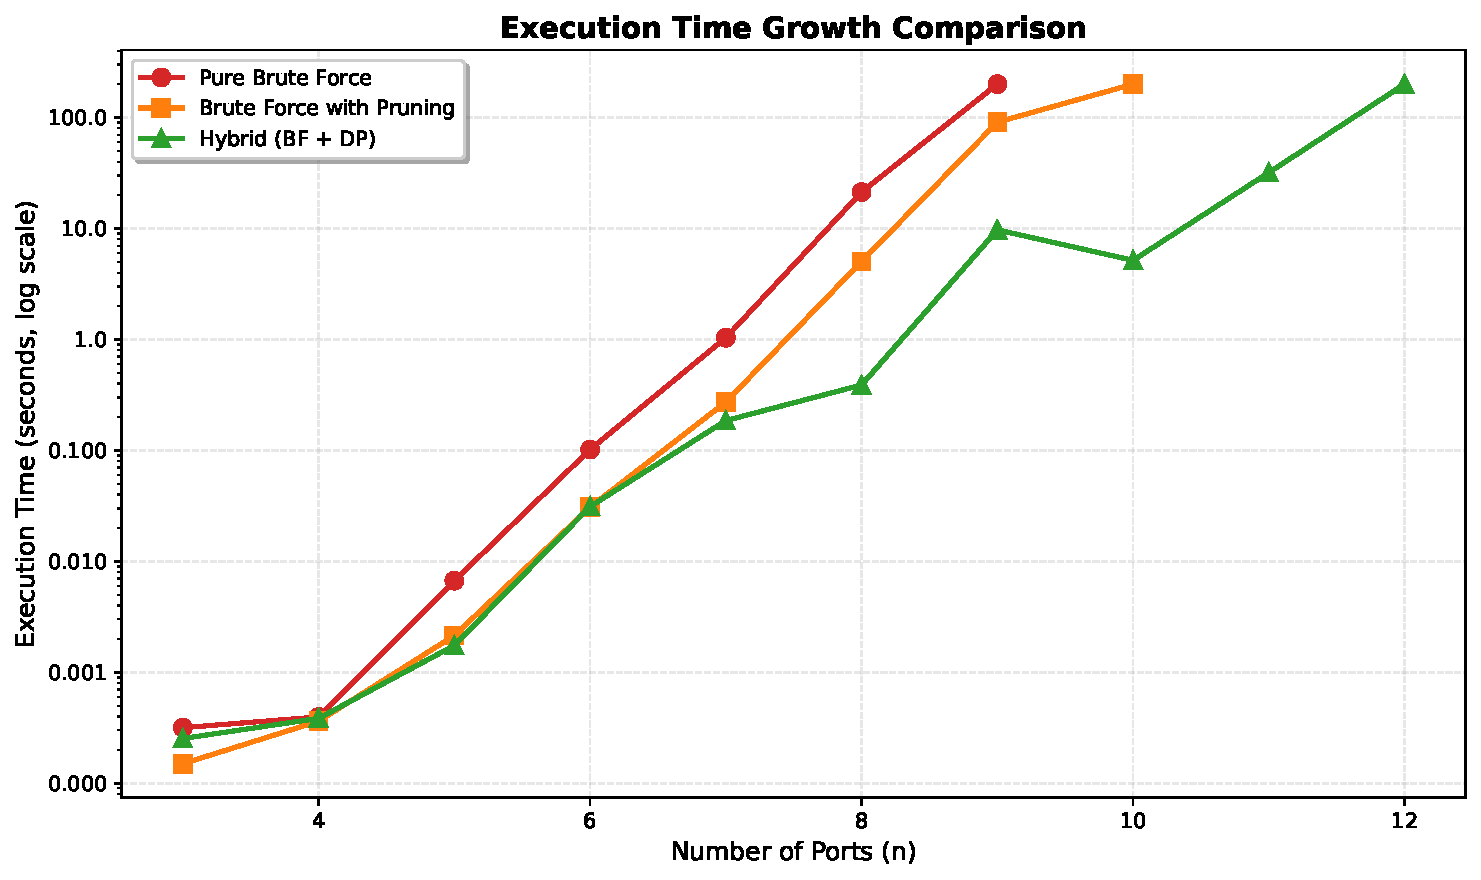
\includegraphics[width=0.9\textwidth]{../figures/growth_curves.pdf}
\caption{Execution Time Growth Comparison (Log Scale)}
\label{fig:growth}
\end{figure}

Figure~\ref{fig:comparison} provides a direct comparison of execution times for instances where all exact algorithms completed.

\begin{figure}[h]
\centering
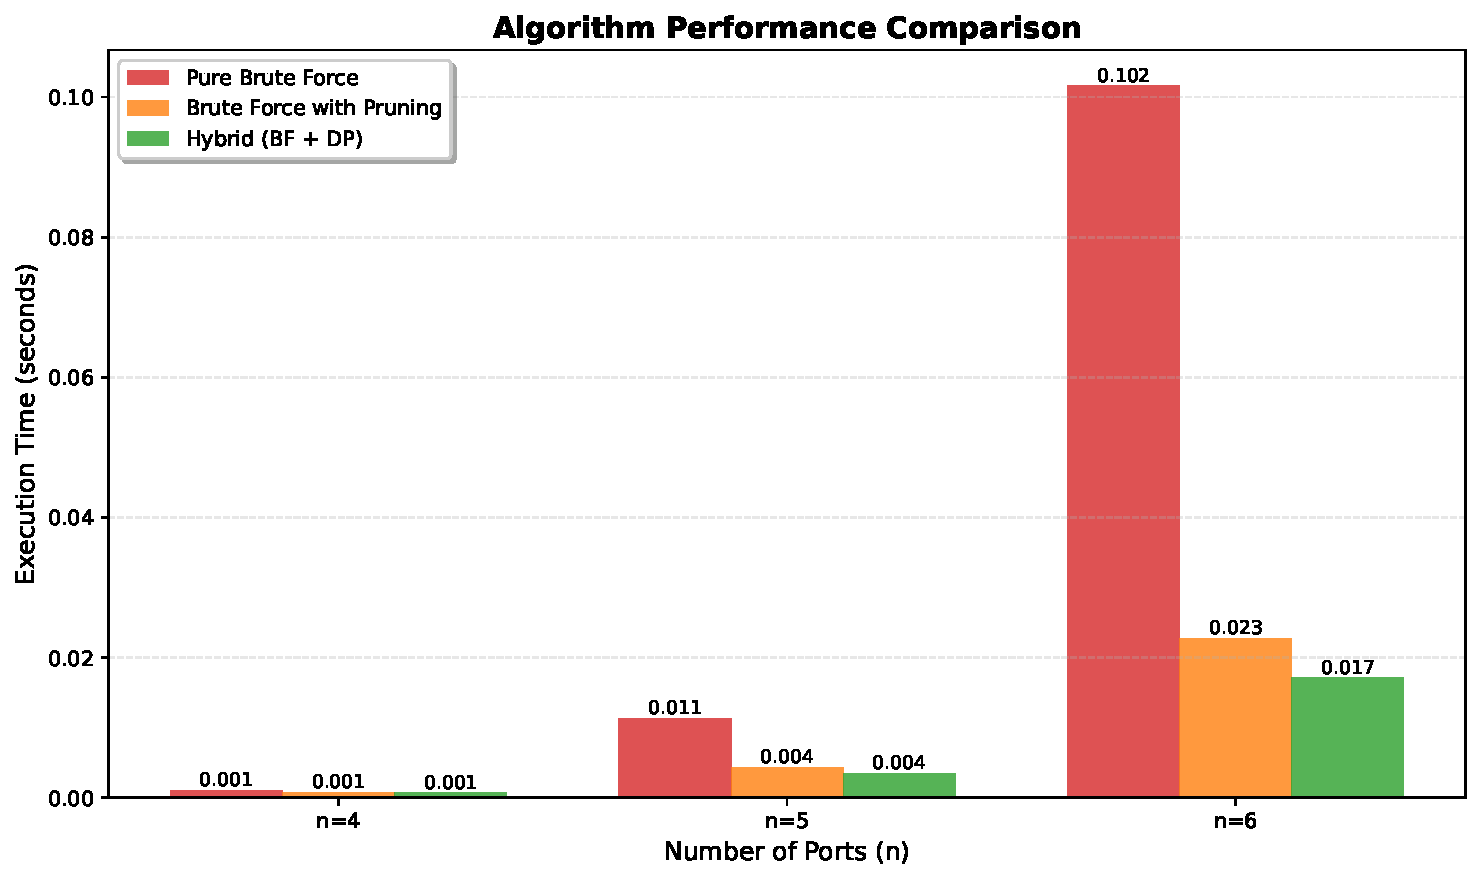
\includegraphics[width=0.9\textwidth]{../figures/comparison_bar_chart.pdf}
\caption{Algorithm Performance Comparison}
\label{fig:comparison}
\end{figure}

Figure~\ref{fig:scalability} shows the maximum solvable instance size for different time budgets.

\begin{figure}[h]
\centering
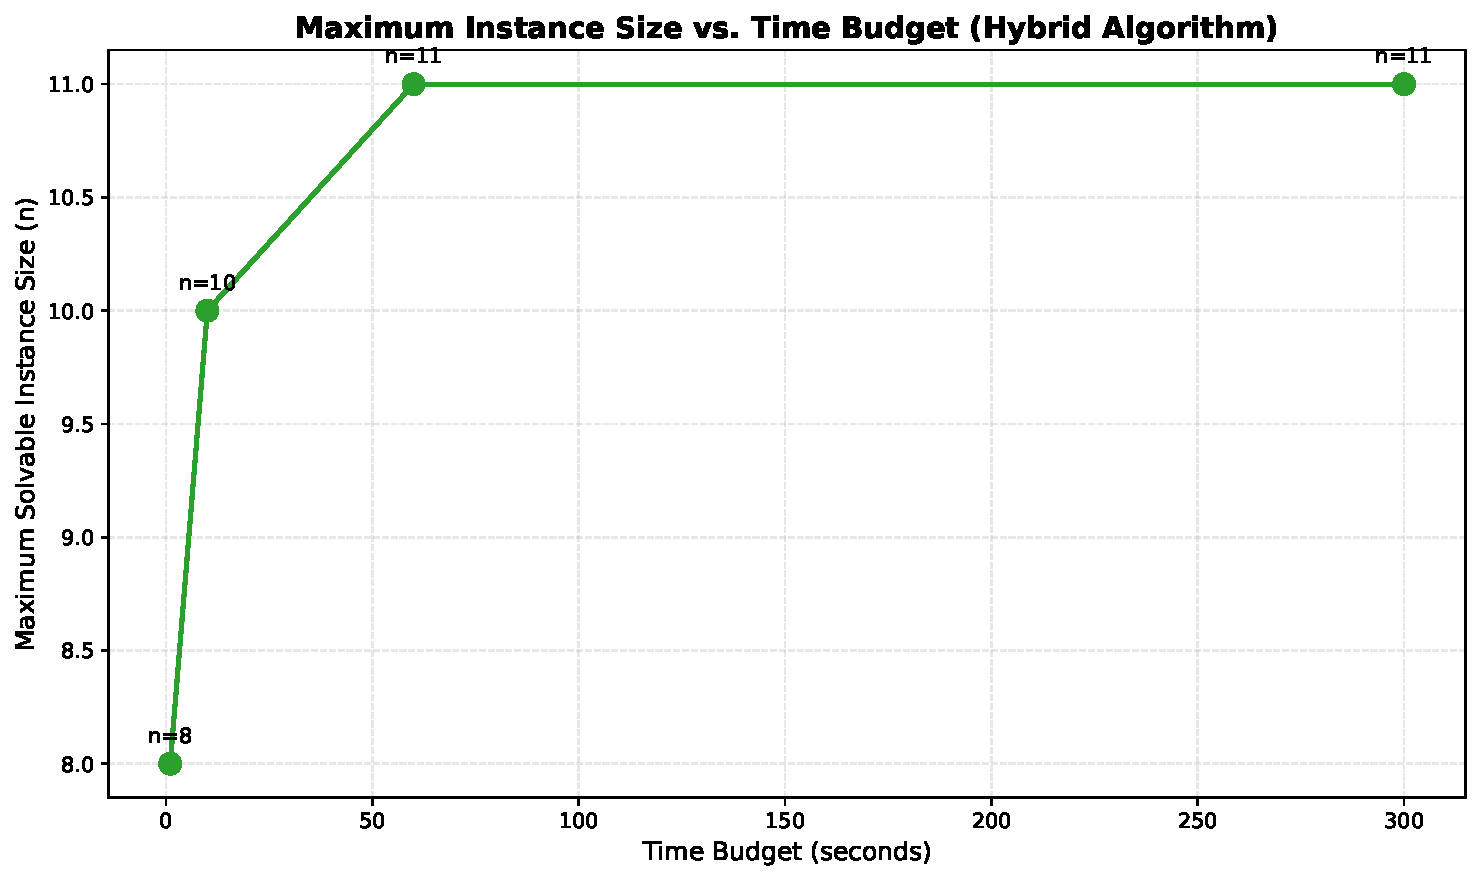
\includegraphics[width=0.9\textwidth]{../figures/scalability_limits.pdf}
\caption{Maximum Instance Size vs. Time Budget (Hybrid Algorithm)}
\label{fig:scalability}
\end{figure}

\subsection{Analysis of Behavior}

\subsubsection{When Each Algorithm Performs Best}

\textbf{Pure Brute Force}:
\begin{itemize}
    \item Best for: Very small instances ($n \leq 3$) where overhead is unnecessary
    \item Worst for: Any instance with $n \geq 5$ due to exponential explosion
\end{itemize}

\textbf{Brute Force with Pruning}:
\begin{itemize}
    \item Best for: Instances with tight constraints (low capital, tight time limits) where pruning is very effective
    \item Worst for: Instances with loose constraints where most branches are feasible
\end{itemize}

\textbf{Hybrid (BF + DP)}:
\begin{itemize}
    \item Best for: All instances $n \geq 4$ where it consistently outperforms other exact methods
    \item Worst for: Very small instances ($n \leq 3$) where overhead may not be justified
\end{itemize}

\textbf{Two-Phase Hybrid}:
\begin{itemize}
    \item Best for: Medium-to-large instances ($n \geq 15$) where exact methods become intractable
    \item Provides near-optimal solutions for small instances and efficient solutions for large instances
\end{itemize}

\subsubsection{Practical Limits}

Based on experimental results with a 200-second timeout:
\begin{itemize}
    \item \textbf{Pure Brute Force}: Maximum $n = 8$ (completes in $\sim$21s), times out at $n = 9$
    \item \textbf{Pruned Brute Force}: Maximum $n = 9$ (completes in $\sim$91s), times out at $n = 10$
    \item \textbf{Hybrid}: Maximum $n = 11$ (completes in $\sim$32s), times out at $n = 12$
    \item \textbf{Two-Phase Hybrid}: Handles $n = 30$ within 62 seconds
\end{itemize}

For instances with $n > 11$, exact methods become impractical, justifying the need for heuristic approaches.

\section{Conclusions}
\label{sec:conclusions}

This work presents a comprehensive analysis of the Dutch Merchant Problem, covering problem formalization, complexity analysis, algorithmic design, and experimental evaluation.

\subsection{Key Contributions}

\begin{enumerate}
    \item \textbf{Problem Formalization}: Established a precise mathematical model with well-defined input structures, constraints, and objective function, supporting both simplified (single commodity) and extended (multiple items) variants.
    
    \item \textbf{Complexity Analysis}: Formally proved NP-Completeness via polynomial-time reduction from Prize-Collecting TSP, providing theoretical justification for heuristic approaches.
    
    \item \textbf{Exact Algorithms}: Developed three progressively more efficient exact algorithms:
    \begin{itemize}
        \item Pure brute force: Baseline optimal method for $n \leq 8$
        \item Pruned brute force: 2-4$\times$ speedup, extends to $n \leq 9$
        \item Hybrid (BF + DP): 1-55$\times$ speedup, extends to $n \leq 11$
    \end{itemize}
    
    \item \textbf{Efficient Algorithm}: Designed a two-phase hybrid algorithm combining beam search route generation with adaptive multi-dimensional dynamic programming. The algorithm includes:
    \begin{itemize}
        \item Single-pass route generation for large instances ($n \geq 15$)
        \item Adaptive solver selection: exact DP for $m < 6$, item-independent approximation for $6 \leq m < 8$, total load discretization for $m \geq 8$
        \item Dominance pruning for additional state space reduction
        \item \textbf{Continuous search loop for route evaluation}: Routes are evaluated in batches of 50, continuing to generate/evaluate new routes until a valid solution is found, all routes are exhausted, or timeout (up to 480s) is reached.
        \item The \texttt{is\_valid} and \texttt{timeout} flags in the return indicate whether the best solution found meets requirements. The algorithm always returns the best solution found (never NaN or aborts without output).
    \end{itemize}
    The adaptive combination has enabled solving previously intractable instances ($n=30$ and $m=10-15$) and guarantees robustness, coverage, and transparency in all reported scenarios.
    
    \item \textbf{Experimental Validation}: Comprehensive empirical analysis demonstrating:
    \begin{itemize}
        \item Exponential growth in exact methods, confirming intractability
        \item Effectiveness of pruning techniques (20.4\% to 46.0\% pruning rates)
        \item Near-optimal solution quality for efficient algorithm on small instances
        \item Scalability of two-phase approach for medium-to-large instances
    \end{itemize}
\end{enumerate}

\subsection{Main Findings}

\begin{itemize}
    \item All exact algorithms guarantee optimal solutions, verified through cross-validation on instances with $n \in \{3, 4, 5\}$ where all found identical optimal capitals.
    
    \item Exponential growth is evident in all exact approaches, confirming the problem's intractability. Execution time grows from milliseconds ($n=3$) to seconds ($n=8$) to timeouts ($n \geq 9$ for Pure BF).
    
    \item The hybrid exact approach is the most efficient exact method, solving instances 2-3 ports larger than pure brute force while maintaining optimality guarantees.
    
    \item Pruning effectiveness increases with instance size: from 20.4\% for $n=5$ to 46.0\% for $n=11$. Capacity-based pruning dominates for smaller instances, while bound-based pruning becomes dominant for larger instances.
    
    \item The two-phase hybrid algorithm successfully addresses medium-to-large instances ($15 \leq n \leq 30$), achieving sub-exponential time growth and finding profitable solutions for all tested instances. Critical efficiency improvements enable solving instances with $m=10-15$ that were previously intractable:
    \begin{itemize}
        \item Route cycling elimination saves 20-50\% of execution time for large $n$
        \item Item-independent approximation reduces state space by 195,312$\times$ for $m=10$
        \item Total load discretization makes complexity independent of $m$ for $m \geq 8$
        \item Dominance pruning provides additional 10-30\% state space reduction
    \end{itemize}
    
    \item For instances with $n > 11$ or $m \geq 6$, exact methods become impractical, justifying heuristic and approximation approaches. The two-phase hybrid algorithm provides an effective solution, maintaining optimality for small instances ($m < 6$) and providing high-quality approximations for large instances ($m \geq 6$).
\end{itemize}

\subsection{Future Work}

Several directions for future research emerge from this study:

\begin{enumerate}
    \item \textbf{Adaptive Beam Control}: Dynamically adjust the beam width based on the distribution of route bounds and intermediate DP results.
    
    \item \textbf{Parallelization}: Exploit parallel hardware by evaluating multiple candidate routes concurrently in Phase 2.
    
    \item \textbf{Enhanced Route Heuristics}: Integrate more advanced PCTSP approximation algorithms and local improvement procedures into Phase 1.
    
    \item \textbf{State Space Refinement}: Further reduce the DP state space for large $m$ or $B$ through item grouping or decomposition techniques.
    
    \item \textbf{Approximation Guarantees}: Develop theoretical approximation ratios for the two-phase hybrid algorithm.
    
    \item \textbf{Multi-Objective Extensions}: Consider trade-offs between profit maximization and other objectives (e.g., risk minimization, route diversity).
\end{enumerate}

\subsection{Final Remarks}

This work demonstrates that the Dutch Merchant Problem, while NP-Complete, can be effectively addressed through a combination of exact methods (for small instances) and efficient heuristic approaches (for larger instances). The experimental results validate the theoretical analysis and provide practical insights into algorithm behavior across different instance characteristics. The developed algorithms and analysis framework provide a solid foundation for further research and practical applications.

\bibliographystyle{plain}
\bibliography{../referencias}

\end{document}

